% !TeX spellcheck = de_DE
\documentclass{beamer}

\usetheme{Madrid}
\usecolortheme{beaver}

% Navigation Symbols off
\beamertemplatenavigationsymbolsempty{}
%\usenavigationsymbolstemplate{}
\setbeamercolor*{item}{fg=red}
\setbeamercolor{itemize item}{fg=red} % all frames will have red bullets
% Watermark
\usebackgroundtemplate{%
	\rule{0pt}{\paperheight}%
	\hspace*{\paperwidth}%
	\makebox[0pt][r]{\includegraphics[width=60mm]{\resWatermark}}}

\usepackage[utf8]{inputenc}
\usepackage[german]{babel}
\usepackage{latexsym}
\usepackage{stmaryrd}
\usepackage{amsmath}
\usepackage{amssymb}
\usepackage{amsxtra}
\usepackage{amsthm}
\usepackage{hyperref}
\usepackage{graphicx}
\usepackage{tikz}
\usepackage[square,sort,comma,numbers]{natbib}

% Logos
\newcommand{\resLogo}{../images/logo}
\newcommand{\resFBI}{../images/logo_fbi}
\newcommand{\resLogoSingle}{../images/logo_uhh}
\newcommand{\resWatermark}{../images/watermark}

% Custom commands
\newcommand{\gqq}[1]{\glqq#1\grqq} % encloses words in German quotes

\title{Ansätze und Verfahren der Datenmigration}
\subtitle{Datenmigration im Kontext des Reengineering}
\author[Schenkemeyer, Fechner]{\includegraphics[height=1cm]{\resLogo}\\Julian Schenkemeyer, Tobias Fechner\\ \texttt{\footnotesize\{5schenke,1fechner\}@informatik.uni-hamburg.de}}
\institute[UHH]{Universität Hamburg}
\date{\today}

% === DOCUMENT ===
\begin{document}
	
	% === TITLE ===
	\begin{frame}
		\maketitle
	\end{frame}
	
	\addtobeamertemplate{frametitle}{}{%
		\begin{tikzpicture}[remember picture, overlay]
		\node[anchor=north east,yshift=2pt, xshift=2pt] at (current page.north east) {%
			\includegraphics[height=.75cm]{\resFBI}\hspace{3pt}%
			\includegraphics[height=.75cm]{\resLogoSingle}%
		};
		\end{tikzpicture}
	}
	
	% === AGENDA ===
	
	\begin{frame}
		\frametitle{Agenda}
		\tableofcontents
	\end{frame}
	
	% ===========================================================================================================
	% ======= BEGIN CONTENT =====================================================================================
	% ===========================================================================================================
	
	\section{Datenmigration im Kontext des Reengineering}
	
	\begin{frame}
		\frametitle{Datenmigration}
		
		\textit{''Data migration is the selection, perparation, extraction, transformation and
		permanent movement of appropriate data that is of the right quality to the
		right place at the right time and the decommissioning of legacy data stores''} \cite{morris-2012}
	\end{frame}
	
	\begin{frame}
		\frametitle{H"aufige Riskien der Datenmigration}
		
		\begin{itemize}
			\item Technologiezentrierung
			\item Mangel an Spezialisten
			\item Unterschätzen der Datenmigration
			\item Problemzuweisung
		\end{itemize}
	\end{frame}
	
	% ===========================================================================================================
	\section{Generelles Vorgehen}
	
	% ===========================================================================================================
	\section{Strategien zur Datenmigration}
	
	\begin{frame}
		\frametitle{Stratgien}
		
		\begin{itemize}
			\item Strategien auf unterschiedlichen Ebenen
			\item "Anderungen in Daten ziehen "Anderungen in nutzenden Anwendungen nach sich
			\item Ziel ist die Erhaltung von Daten
			\item Unterschiedliche Schwerpunkte erfordern unterschiedliches technisches und fachliches Wissen
		\end{itemize}
	\end{frame}
	
	\subsection{Datenbankebene}
	
	\begin{frame}
		\frametitle{Datenbankebene}
		
		\begin{itemize}
			\item \textbf{Physisch} \\
			TODO %TODO
			\item \textbf{Konzeptuell} \\
			TODO %TODO
		\end{itemize}
	\end{frame}	
	
	\begin{frame}
		\frametitle{Konzeptuelle Konvertierung}
		
		\centering
		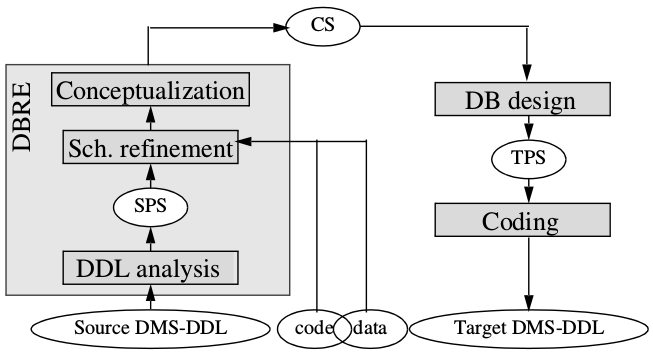
\includegraphics[height = 6cm]{../images/strategies_fig_02b.png}\\
		\tiny Quelle: \cite{henrard-2002}
	\end{frame}
	
	\subsection{Anwendungsebene}
	
	\begin{frame}
		\frametitle{Anwendungsebene}
		
		\begin{itemize}
			\item \textbf{Einsatz eines Wrappers} \\
				TODO %TODO
			\item \textbf{Anpassung von Statements} \\
				TODO %TODO
			\item \textbf{Anpassung der Zugriffslogik} \\
				TODO %TODO
		\end{itemize}
	\end{frame}
	
	\begin{frame}
		\frametitle{Vorgeen zur Einf"uhrung eines Wrappers}
		
		\centering
		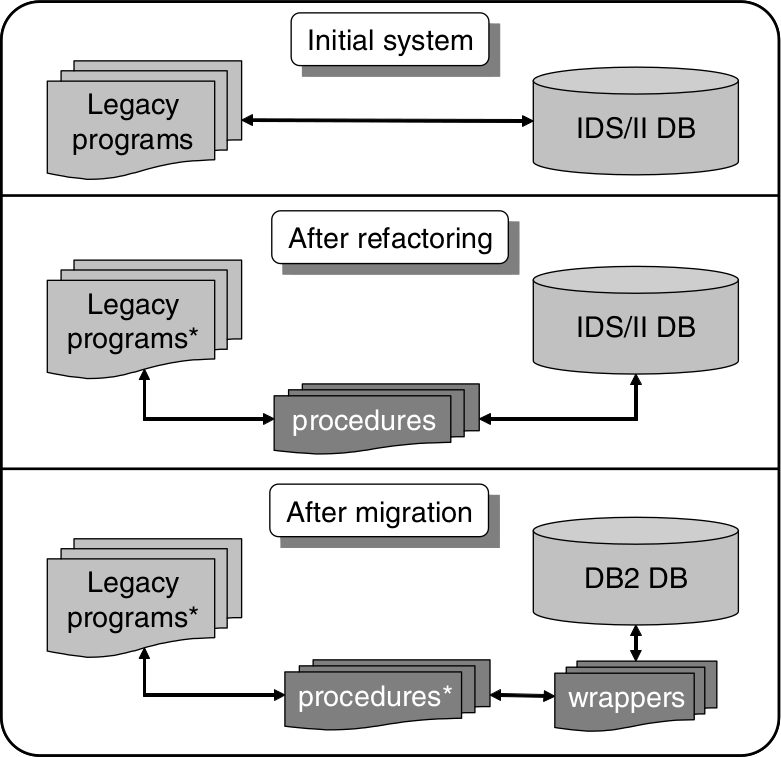
\includegraphics[height = 7cm]{../images/large_scale_fig_01.png} \\
		\tiny Quelle: \cite{henrard-2008}
	\end{frame}
	
	% ===========================================================================================================
	\section{Einf"uhrungsstrategien der Datenmigration}
	
	\subsection{Big-Bang-Ansatz}
	
	%TODO
	
	\subsection{Chicken-Little-Ansatz}
	
	%TODO
	
	\subsection{Butterfly-Ansatz}
	
	%TODO
	
	% ===========================================================================================================
	\section{Fazit}
	
	\begin{frame}
		\frametitle{Fazit}
		
		\begin{itemize}
			\item TODO %TODO
		\end{itemize}
	\end{frame}
	
	% ===========================================================================================================
	% ======= END CONTENT =======================================================================================
	% ===========================================================================================================
	
	% === QUELLEN ===
	%    \section{Quellen}
	
	\begin{frame}
		\frametitle{Quellen}
						
		\bibliographystyle{plaindin}
		\bibliography{../bib/mproj}
	\end{frame}
	
\end{document}
